\section{Entrenamiento con Deepfish}
Esta sección detalla el proceso de entrenamiento de modelos de segmentación utilizando la base de datos Deepfish. Se emplearon modelos preentrenados en la base de datos COCO, disponibles en la plataforma Ultralytics, y se ajustaron mediante re-entrenamiento para adaptarlos a la tarea específica de segmentación de peces en el entorno marino. Además este entrenamiento sirve como plantilla para los entrenamientos posteriores con la base de datos de salmones.

\subsection{Entrenamiento inicial}
El objetivo de este entrenamiento es evaluar el rendimiento de los modelos al aplicarlos directamente a la base de datos Deepfish, sin realizar ajustes adicionales. Esto permite establecer una línea base para encaminar los entrenamientos posteriores con búsqueda de hiperparámetros y optimización.

Se entrenaron modelos YOLO de segmentación en diferentes tamaños y versiones, los modelos entrenados son: YOLOv8n, YOLOv8s, YOLOv8m, YOLOv8l, YOLOv8x, YOLOv9c, YOLOv9e, YOLO11n, YOLO11s, YOLO11m, YOLO11l y YOLO1x. Para cada modelo se utilizaron las versiones completa y ``_LO'' de la base de datos Deepfish, con el objetivo de evaluar el impacto de las imágenes de fondo en el rendimiento del modelo. Se realizaron entrenamientos completos (sin congelar capas) y entrenamientos con TL \textit{(Transfer Learning)} (congelando capas del \textit{backbone} según se ve en la tabla \ref{tab:models_summary_freeze}). Además para cada variante de entrenamiento se realizó una versión utilizando el optimizador AdamW y otra con SGD. Cada entrenamiento fue de 80 épocas y se utilizaron hiperparámetros por defecto de Ultralytics. En total se realizaron 48 entrenamientos.

\begin{table}[htbp]
\centering
\caption[Sumario de modelos YOLO a entrenar]{Resumen de cada modelo: capas totales, parámetros, gradients, GFLOPs y número de capas del \textit{backbone} congeladas al realizar TL.}
\label{tab:models_summary_freeze}
\resizebox{\textwidth}{!}{
\begin{tabular}{|l|r|r|r|r|c|}
\hline
\textbf{Modelo} & \textbf{Capas} & \textbf{Parámetros} & \textbf{Gradients} & \textbf{GFLOPs} & \textbf{Backbone} \\ \hline
yolov8n-seg  & 151 & 3,263,811  & 3,263,795  & 12.1  & 10 \\ \hline
yolov8s-seg  & 151 & 11,790,483 & 11,790,467 & 42.7  & 10 \\ \hline
yolov8m-seg  & 191 & 27,240,227 & 27,240,211 & 110.4 & 10 \\ \hline
yolov8l-seg  & 231 & 45,936,819 & 45,936,803 & 220.8 & 10 \\ \hline
yolov8x-seg  & 231 & 71,751,811 & 71,751,795 & 344.5 & 10 \\ \hline
yolov9c-seg  & 380 & 27,836,211 & 27,836,195 & 159.1 & 10 \\ \hline
yolov9e-seg  & 743 & 60,451,891 & 60,451,875 & 248.1 & 30 \\ \hline
yolo11n-seg  & 203 & 2,842,803  & 2,842,787  & 10.4  & 11 \\ \hline
yolo11s-seg  & 203 & 10,082,675 & 10,082,659 & 35.6  & 11 \\ \hline
yolo11m-seg  & 253 & 22,359,987 & 22,359,971 & 123.6 & 11 \\ \hline
yolo11l-seg  & 379 & 27,617,459 & 27,617,443 & 142.7 & 11 \\ \hline
yolo11x-seg  & 379 & 62,051,411 & 62,051,395 & 319.7 & 11 \\ \hline
\end{tabular}
}
\end{table}

\subsubsection{Efecto del tamaño del modelo}
Se observa que en métricas como F1 y mAP@50 el aumento de tamaño no garantiza mejora (fig. \ref{fig:deepfish_yolov8_metrics_stacked}): los modelos pequeños (n, s) rinden peor, la ganancia se atenúa a partir de los tamaños medianos-grandes (m, l) ---probablemente por la complejidad limitada de Deepfish y el riesgo de sobreajuste. En cambio, usando la métrica más exigente mAP@50-95 (fig. \ref{fig:deepfish_yolov8_metrics_stacked} y \ref{fig:deepfish_yolo9_yolo11_metrics_map50_95}) los modelos grandes sí muestran una mejora consistente, indicando mejor captura de detalles finos en la segmentación.

Para este análisis se excluyeron \textit{outliers} de muy bajo rendimiento ($\text{F1} < 0.6$) atribuidos a entrenamientos puntuales con AdamW, esto se analiza más adelante.

\begin{figure}[htbp]
  \centering
  \begin{subfigure}[b]{\textwidth}
    \centering
    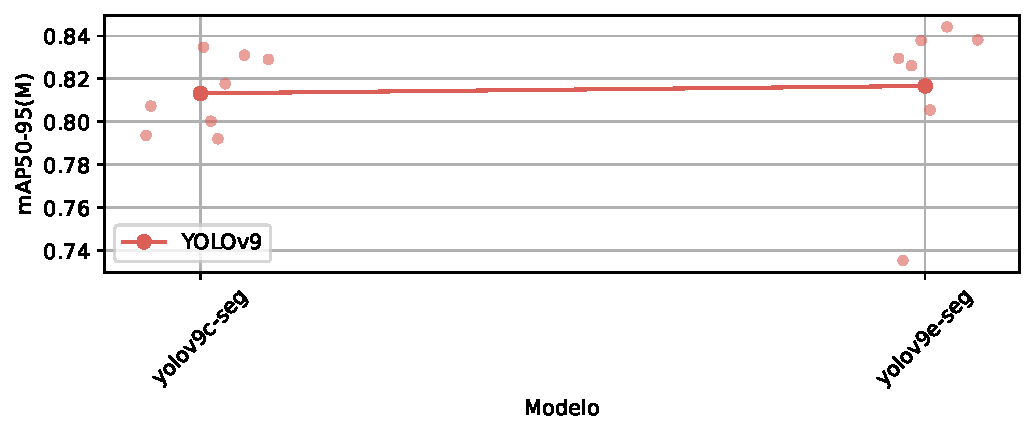
\includegraphics[width=0.9\textwidth]{figures/DeepFish-sizeComparison-YOLOv9-mAP50-95(M).pdf}
    \caption{Puntaje mAP@50-95 promedio obtenido por modelos YOLOv9 en Deepfish.}
    \label{fig:deepfish_yolov9_map50_95}
  \end{subfigure}

  \begin{subfigure}[b]{\textwidth}
    \centering
    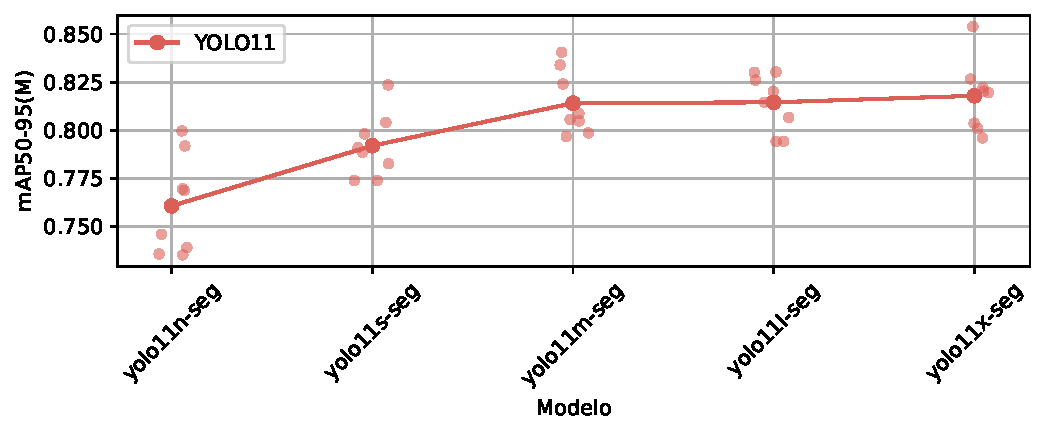
\includegraphics[width=0.9\textwidth]{figures/DeepFish-sizeComparison-YOLO11-mAP50-95(M).pdf}
    \caption{Puntaje mAP@50-95 promedio obtenido por distintos modelos YOLOv9 en Deepfish.}
    \label{fig:deepfish_yolo11_map50_95}
  \end{subfigure}
  \caption[Puntaje mAP@50-95 de los modelos YOLOv9 y YOLO11 para Deepfish]{Comparación del puntaje mAP@50-95 para distintos tamaños de modelos YOLOv9 y YOLO11 en Deepfish.}
  \label{fig:deepfish_yolo9_yolo11_metrics_map50_95}
\end{figure}

\begin{figure}[htbp]
  \centering
  \begin{subfigure}[b]{\textwidth}
    \centering
    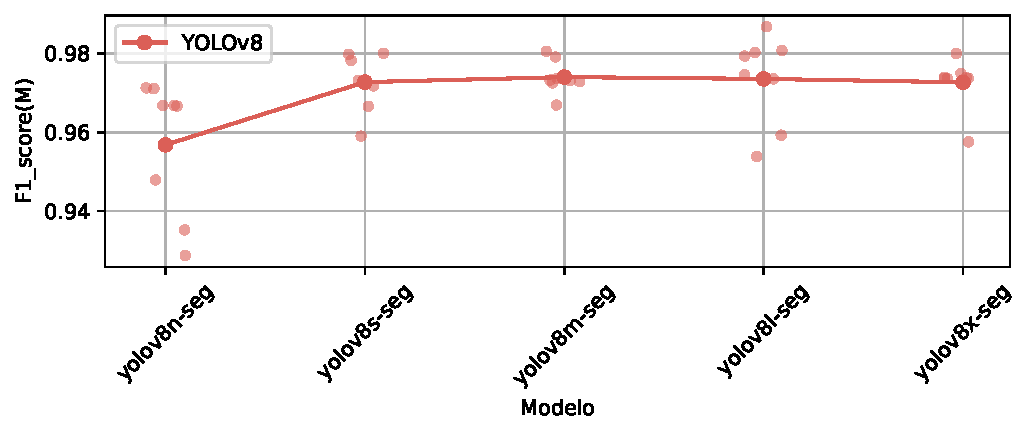
\includegraphics[width=0.9\textwidth]{figures/DeepFish-sizeComparison-YOLOv8-F1_score(M).pdf}
    \caption{Puntaje F1 promedio obtenido por distintos modelos YOLOv8 en Deepfish.}
    \label{fig:deepfish_yolov8_f1}
  \end{subfigure}

  \begin{subfigure}[b]{\textwidth}
    \centering
    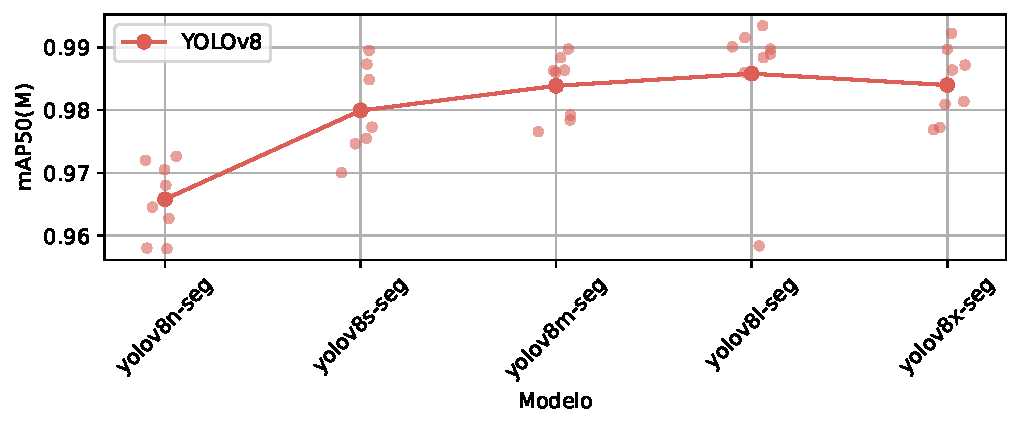
\includegraphics[width=0.9\textwidth]{figures/DeepFish-sizeComparison-YOLOv8-mAP50(M).pdf}
    \caption{Puntaje mAP@50 promedio obtenido por distintos modelos YOLOv8 en Deepfish.}
    \label{fig:deepfish_yolov8_map50}
  \end{subfigure}

  \begin{subfigure}[b]{\textwidth}
    \centering
    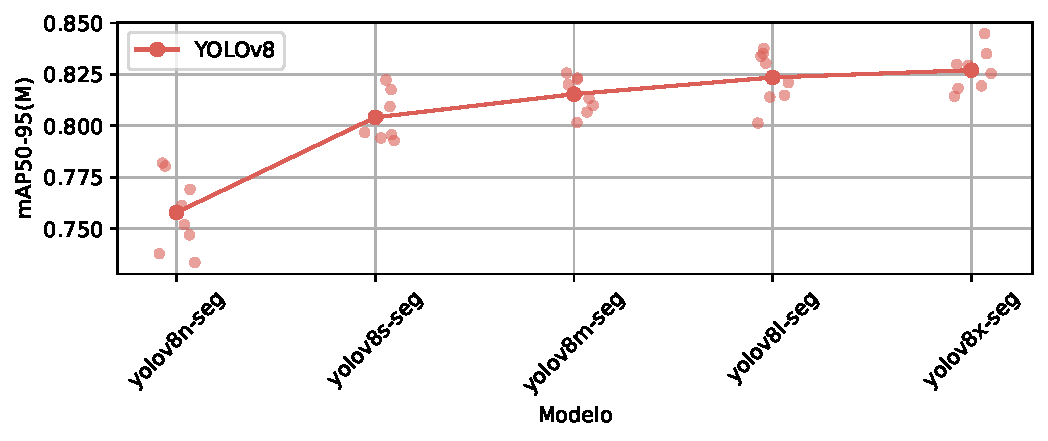
\includegraphics[width=0.9\textwidth]{figures/DeepFish-sizeComparison-YOLOv8-mAP50-95(M).pdf}
    \caption{Puntaje mAP@50-95 promedio obtenido por distintos modelos YOLOv8 en Deepfish.}
    \label{fig:deepfish_yolov8_map50_95}
  \end{subfigure}

  \caption[Comparación de métricas por tamaño de modelo YOLOv8 en Deepfish]{Comparación vertical de las métricas F1_score, mAP@50 y mAP@50-95 para distintos tamaños de modelos YOLOv8 en Deepfish.}
  \label{fig:deepfish_yolov8_metrics_stacked}
\end{figure}

\subsubsection{Efecto del Transfer Learning}
Entrenar por medio de TL resulta en promedio en mejoras marginales en F1 y mAP@50 pero demuestra un peor rendimiento en mAP@50-95 (fig. \ref{fig:deepfish_yolo_TL_metrics_stacked}). Esto sugiere que congelar el \textit{backbone} limita la capacidad del modelo para adaptarse a los detalles específicos de la segmentación de peces, afectando negativamente la precisión en umbrales más estrictos pero sin impactar significativamente en métricas más generales. Se ignoraron \textit{outliers} para este análisis.

Además ---como se ve más adelante--- el entrenamiento con TL mostró una mayor caída en el rendimiento al utilizar modelos exportados con TensorRT (fig. \ref{fig:deepfish_yolo_format_factor_mejora}).

\subsubsection{Efecto del optimizador}
El uso de diferentes optimizadores puede influir en el rendimiento del modelo. En este estudio, se compararon los optimizadores AdamW y SGD, encontrando que SGD consistentemente supera a AdamW en todas las métricas evaluadas (fig. \ref{fig:deepfish_yolo_optimizer_map50_95}). AdamW mostró un rendimiento ligeramente más bajo en múltiples entrenamientos, con varios casos \textit{outliers} que sugieren problemas de convergencia o ajuste inadecuado a la tarea específica de segmentación para esta base de datos. Estas diferencias se acrecentan aún más para modelos exportados con TensorRT y cuantización numerica INT8 (tabla \ref{tab:deepfish_factorMejora_optimizer}).

\begin{table}[htbp]
\centering
\caption[Factor de mejora entre SGD y AdamW en Deepfish]{Factor de mejora promedios entre SGD y AdamW, por formato de exportación, con y sin incluir \textit{outliers}. Valores mayores a 1 indican que SGD supera a AdamW.}
\label{tab:deepfish_factorMejora_optimizer}
\resizebox{\textwidth}{!}{
\begin{tabular}{|l|l|l|l|l|l|l|}
\hline
\textbf{Precision} & \textbf{Recall} & \textbf{F1\_score} & \textbf{mAP50} & \textbf{mAP50-95} & \textbf{Format} & \textbf{Outliers} \\ \hline
1.001500 & 1.004742 & 1.003064 & 1.002672 & 1.018452 & Pytorch & False \\ \hline
0.998262 & 1.004581 & 1.001264 & 1.002028 & 1.017949 & TensorRT-F32 & False \\ \hline
0.997701 & 1.004935 & 1.001163 & 1.001703 & 1.017562 & TensorRT-F16 & False \\ \hline
1.029502 & 1.058339 & 1.043069 & 1.025606 & 1.050564 & TensorRT-INT8 & False \\ \hline
1.006372 & 1.017498 & 1.011638 & 1.007717 & 1.025736 & Promedio & False \\ \hline
1.016525 & 1.022879 & 1.019664 & 1.023022 & 1.065295 & Pytorch & True \\ \hline
1.015045 & 1.022715 & 1.018741 & 1.021350 & 1.064378 & TensorRT-F32 & True \\ \hline
1.014581 & 1.023062 & 1.018684 & 1.021035 & 1.064082 & TensorRT-F16 & True \\ \hline
1.166342 & 1.221879 & 1.197823 & 1.312258 & 1.629470 & TensorRT-INT8 & True \\ \hline
1.053123 & 1.072634 & 1.063728 & 1.094416 & 1.205806 & Promedio & True \\ \hline
\end{tabular}
}
\end{table}

Estos resultados indican que SGD es una opción más robusta y efectiva para este tipo de tareas en comparación con AdamW.

\begin{figure}[htbp]
  \centering
  \begin{subfigure}[b]{\textwidth}
    \centering
    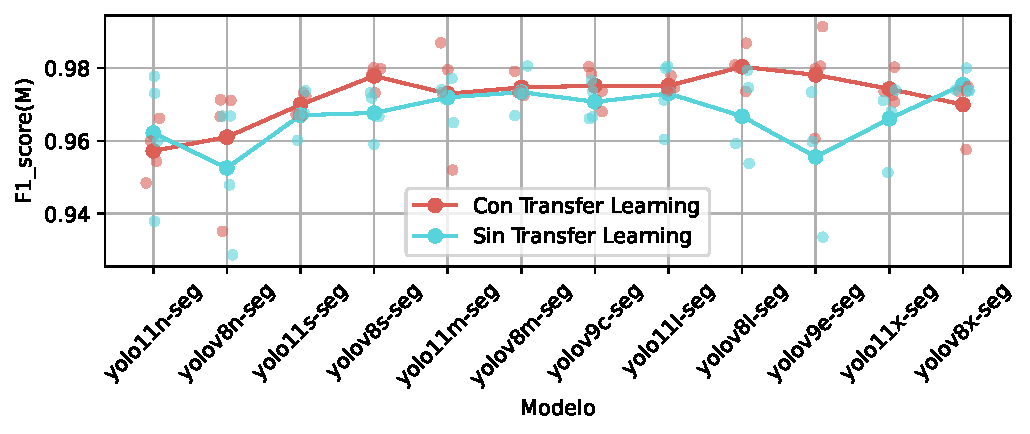
\includegraphics[width=0.9\textwidth]{figures/DeepFish-TransferLearningComparison-YOLO-F1_score(M).pdf}
    \caption{Puntaje F1 promedio obtenido por distintos modelos YOLO en Deepfish con y sin TL.}
    \label{fig:deepfish_yolo_TL_f1}
  \end{subfigure}

  \begin{subfigure}[b]{\textwidth}
    \centering
    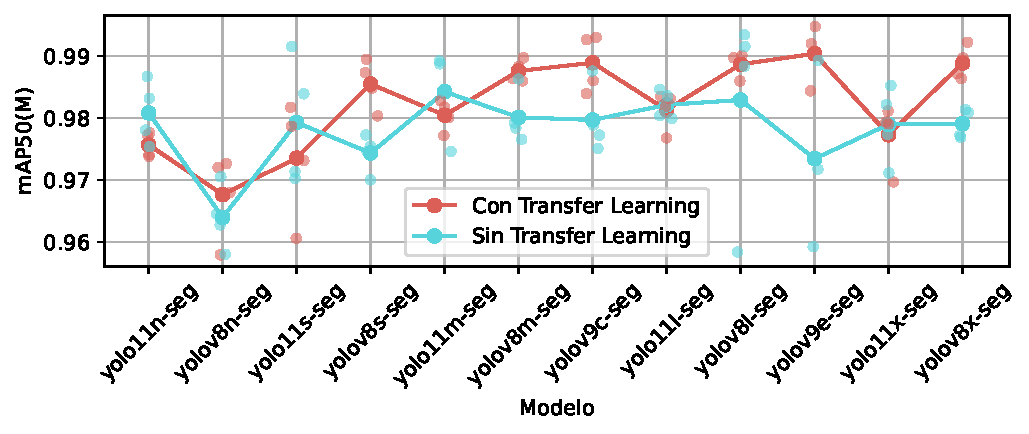
\includegraphics[width=0.9\textwidth]{figures/DeepFish-TransferLearningComparison-YOLO-mAP50(M).pdf}
    \caption{Puntaje mAP@50 promedio obtenido por distintos modelos YOLO en Deepfish con y sin TL.}
    \label{fig:deepfish_yolo_TL_map50}
  \end{subfigure}

  \begin{subfigure}[b]{\textwidth}
    \centering
    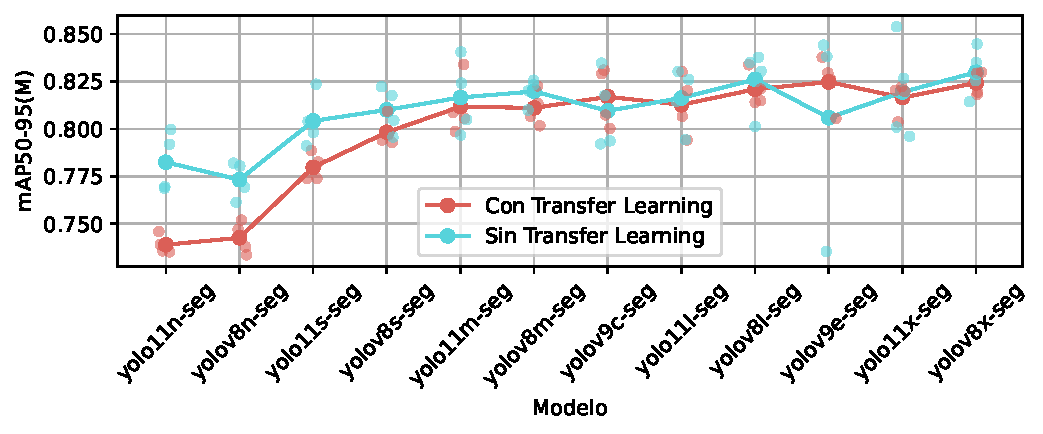
\includegraphics[width=0.9\textwidth]{figures/DeepFish-TransferLearningComparison-YOLO-mAP50-95(M).pdf}
    \caption{Puntaje mAP@50-95 promedio obtenido por distintos modelos YOLO en Deepfish con y sin TL.}
    \label{fig:deepfish_yolo_TL_map50_95}
  \end{subfigure}

  \caption[Comparación de métricas por modelo YOLO en Deepfish con y sin Transfer Learning]{Comparación vertical de las métricas F1_score, mAP@50 y mAP@50-95 para distintos modelos YOLO en Deepfish, con y sin el uso de Transfer Learning.}
  \label{fig:deepfish_yolo_TL_metrics_stacked}
\end{figure}

\begin{figure}[htbp]
  \centering
  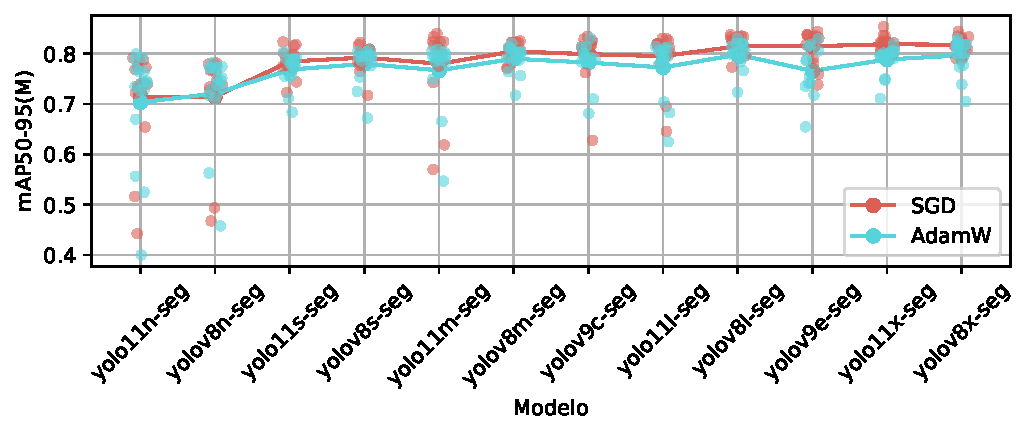
\includegraphics[width=0.9\textwidth]{figures/DeepFish-OptimizerComparison-YOLO-mAP50-95(M).pdf}
  \caption[Puntaje mAP@50-95 de los modelos YOLO con distintos optimizadores]{Comparación del puntaje mAP@50-95 para distintos modelos YOLO en Deepfish, utilizando los optimizadores AdamW y SGD.}
  \label{fig:deepfish_yolo_optimizer_map50_95}
\end{figure}

\subsubsection{Efecto del dataset (Full vs ``LO'')}
Para la base de datos Deepfish, la inclusión de imágenes de fondo suele mejorar de forma marginal el rendimiento de los modelos, aunque no en todos los entrenamientos (tabla \ref{tab:deepfish_mejoraRelativa_model} y fig. \ref{fig:deepfish_yolo_dataset_comparison_map50_95}). Su omisión, además, parece empeorar ligeramente la convergencia, ya que aumenta el número de \textit{outliers} de bajo rendimiento, pero no es un efecto concluyente. En promedio la mejora es de tan solo un 1\%, pero en ciertas circunstancias la diferencia se acrecenta ---ver efecto de exportación.

\begin{table}[htbp]
\centering
\caption[Mejora relativa del uso de imágenes de fondo en Deepfish, por modelo]{Mejora relativa del uso de imágenes de fondo en Deepfish, por modelo. Valores mayores a 1 indican que la versión completa supera a ``LO''.}
\label{tab:deepfish_mejoraRelativa_model}
\begin{tabular}{|l|l|l|l|}
\hline
\textbf{F1\_score} & \textbf{mAP50} & \textbf{mAP50-95} & \textbf{Model} \\ \hline
1.031997 & 1.037910 & 1.047113 & yolo11n-seg \\ \hline
1.035803 & 1.014060 & 1.016982 & yolov8n-seg \\ \hline
0.993440 & 0.985146 & 0.994686 & yolo11s-seg \\ \hline
1.009829 & 1.006209 & 1.017499 & yolov8s-seg \\ \hline
1.015479 & 1.013459 & 1.026629 & yolo11m-seg \\ \hline
0.994692 & 0.999929 & 1.007808 & yolov8m-seg \\ \hline
1.027096 & 1.015316 & 1.033245 & yolov9c-seg \\ \hline
1.010582 & 1.012976 & 1.024967 & yolo11l-seg \\ \hline
0.990465 & 0.988317 & 0.998920 & yolov8l-seg \\ \hline
1.008571 & 1.011124 & 1.017361 & yolov9e-seg \\ \hline
1.003489 & 1.006284 & 1.012529 & yolo11x-seg \\ \hline
1.001750 & 0.997011 & 0.990093 & yolov8x-seg \\ \hline
1.010093 & 1.007110 & 1.015366 & Promedio \\ \hline
\end{tabular}
\end{table}

Otro aspecto relevante a mencionar es que la omisión de imágenes de fondo incrementa la caida de rendimiento al utilizar modelos exportados con TensorRT y cuantización numérica INT8 (fig. \ref{fig:deepfish_yolo_dataset_factor_mejora_by_format}). Esto puede implicar que la presencia de imágenes de fondo ayuda a generalizar el aprendisaje del modelo a lo largo de todo el rango dinámico de pesos y activaciones, lo que se ve reflejado en una menor degradación al aplicar técnicas de optimización numérica agresivas.

\begin{figure}[htbp]
  \centering
  \begin{subfigure}[b]{\textwidth}
    \centering
    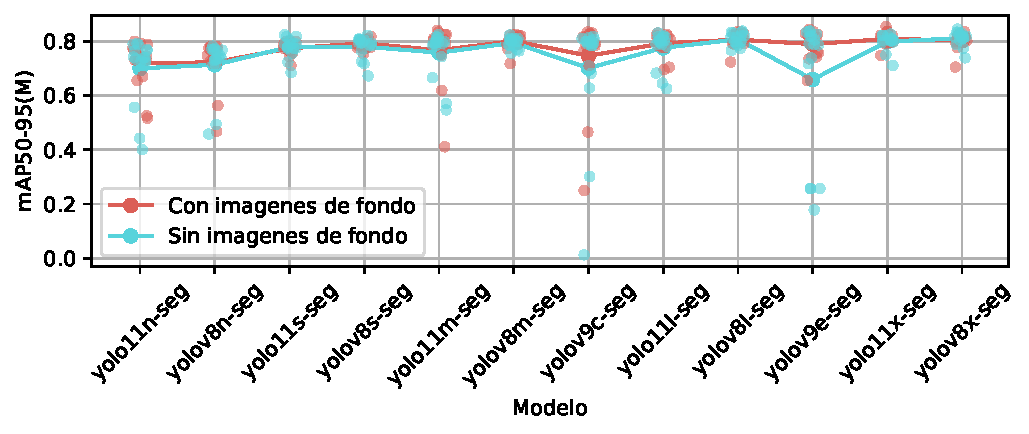
\includegraphics[width=0.9\textwidth]{figures/DeepFish-DatasetComparison-YOLO-mAP50-95(M).pdf}
    \caption{Comparación del puntaje mAP@50-95 entre los \textit{datasets} Full y ``LO'' de Deepfish.}
    \label{fig:deepfish_yolo_dataset_comparison_map50_95}
  \end{subfigure}

  \begin{subfigure}[b]{\textwidth}
    \centering
    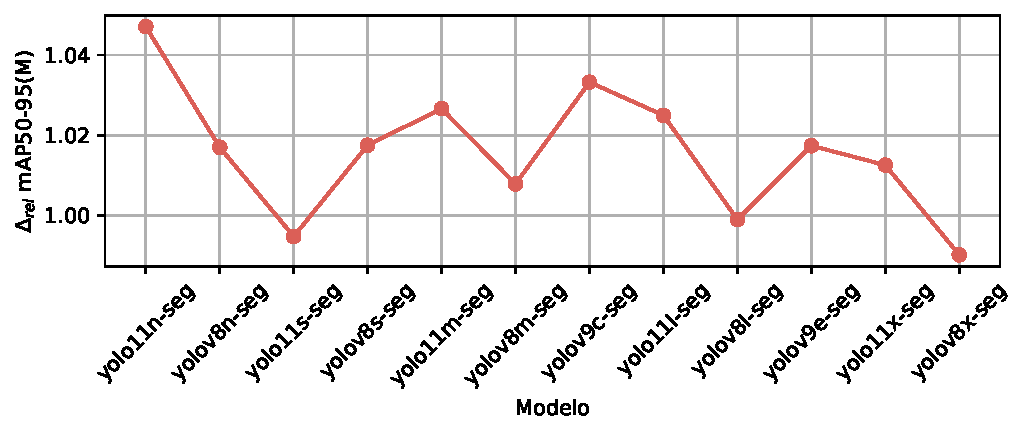
\includegraphics[width=0.9\textwidth]{figures/DeepFish-DatasetFactorMejora-YOLO-mAP50-95(M).pdf}
    \caption{Factor de mejora promedio entre los \textit{datasets} Full y ``LO'' de Deepfish, por modelo. Valores mayores a 1 indican que la versión Full supera a ``LO''.}
    \label{fig:deepfish_yolo_dataset_factor_mejora_by_model}
  \end{subfigure}

  \caption[Comparación del rendimiento entre los \textit{datasets} Full y ``LO'' de Deepfish]{Comparación del rendimiento entre los \textit{datasets} Full y ``LO'' de Deepfish, por modelo.}
  \label{fig:deepfish_yolo_dataset_comparison}
\end{figure}

En conclusión, la inclusión de imágenes de fondo en la base de datos Deepfish tiende a mejorar ligeramente el rendimiento de los modelos entrenados, efecto que se acentúa al aplicar técnicas de optimización numérica con exportación en TensorRT.

\subsubsection{Efecto de la exportación (PyTorch vs TensorRT)}
Con el fin de evaluar el impacto de la optimización y conversión del modelo, se comparan las métricas de evaluación de modelos resultantes obtenidos utilizando el formato nativo de PyTorch con aquellos obtenidos tras la exportación a TensorRT en diferentes precisiones numéricas.

En primera instancia se observa que la exportación a TensorRT en precisión FP32 y FP16 tiene un impacto mínimo en el rendimiento del modelo ($\sim$0.24\% en mAP50 y $\sim$1.1\% en mAP50-95), sin embargo, la cuantización a INT8 resulta en una degradación más significativa ($\sim$7\% en mAP50 y $\sim$12\% en mAP50-95) (tabla \ref{tab:deepfish_mejoraRelativaPromedio_format} y fig. \ref{fig:deepfish_yolo_format_comparison}).

Respecto a tiempos de inferencia, el uso de TensorRT suele mejorar el rendimiento. El incremento en velocidad depende del formato de exportación y tamaño del modelo. En promedio se observa un empeoramiento del 0.73x con FP32 pero mejoras de un 2x con FP16 y 2.7x con INT8 (tabla \ref{tab:deepfish_mejoraRelativaPromedio_format}), aunque con algunos modelos se alcanza un 3x en FP16 y 4x en INT8 (fig. \ref{fig:deepfish_yolo_inference_time_comparison}).

\begin{table}[htbp]
\centering
\caption{Mejora relativa de exportar con TensorRT con diferentes precisiones en Deepfish. Valores menores a 1 indican caída de rendimiento de Pytorch a TensorRT, para tiempos de inferencia es al revés.}
\label{tab:deepfish_mejoraRelativaPromedio_format}
\begin{tabular}{|c|c|c|c|c|}
\hline
\textbf{F1\_score} & \textbf{mAP50} & \textbf{mAP50-95} & \textbf{Inference} & \textbf{Format} \\ \hline
0.998918 & 0.997428 & 0.988555 & 1.324265 & TensorRT-F32 \\ \hline
0.998980 & 0.997606 & 0.989441 & 0.491259 & TensorRT-F16 \\ \hline
0.917626 & 0.929447 & 0.888295 & 0.359059 & TensorRT-INT8 \\ \hline
\end{tabular}
\end{table}

\begin{figure}[htbp]
\begin{center}
    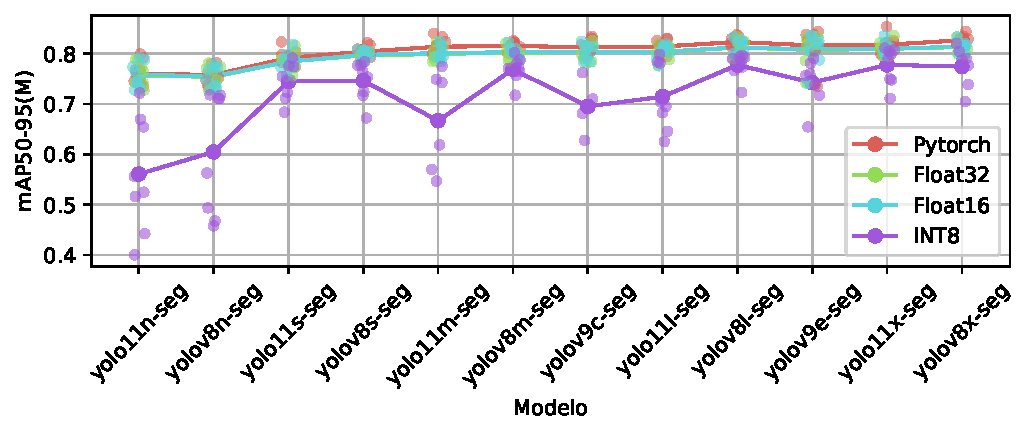
\includegraphics[width=0.9\textwidth]{figures/DeepFish-FormatComparison-YOLO-mAP50-95(M).pdf}
    \caption[Comparación del rendimiento entre los formatos de exportación (PyTorch vs TensorRT) en Deepfish]{Comparación del rendimiento entre los formatos de exportación (PyTorch vs TensorRT) en Deepfish.}
    \label{fig:deepfish_yolo_format_comparison}
\end{center}
\end{figure}

\begin{figure}[htbp]
\begin{center}
    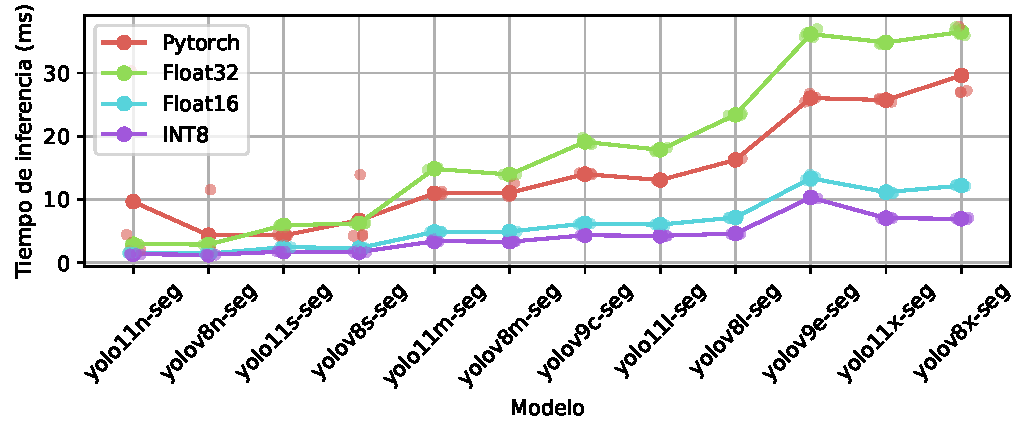
\includegraphics[width=0.9\textwidth]{figures/Deepfish-SpeedComparison-Time-inference.pdf}
    \caption{Comparación de los tiempos de inferencia entre los formatos de exportación (PyTorch vs TensorRT).}
    \label{fig:deepfish_yolo_inference_time_comparison}
\end{center}
\end{figure}

Otro aspecto relevante es la acentuación en la caída de rendimiento al exportar a TensorRT para ciertas configuraciones específicas. Como se menciona en las subsecciones previas, el uso de \textit{Transfer Learning} y la omisión de imágenes de fondo tienden a aumentar la degradación del rendimiento al exportar a TensorRT, especialmente en precisión INT8 (fig. \ref{fig:deepfish_yolo_dataset_factor_mejora_by_format} y \ref{fig:deepfish_yolo_format_factor_mejora}). Este efecto sugiere que estas prácticas pueden limitar la capacidad del modelo para aprender adecuadamente a lo largo de todos sus pesos, lo que se ve reflejado en una mayor pérdida de precisión al aplicar técnicas de optimización.

\begin{figure}[htbp]
\begin{center}
    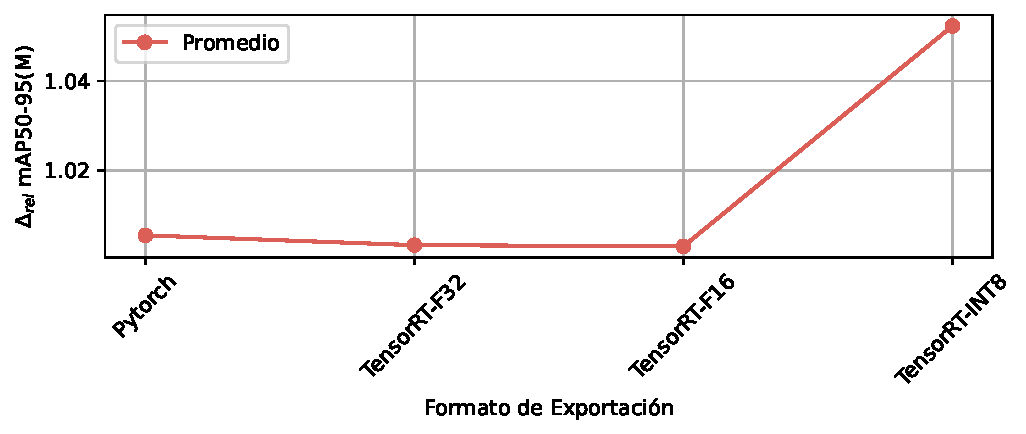
\includegraphics[width=0.9\textwidth]{figures/DeepFish-DatasetFactorMejora-Format-mAP50-95(M).pdf}
    \caption{Factor de mejora entre los \textit{datasets} Full y ``LO'' de Deepfish, por formato de exportación. Valores mayores a 1 indican que la versión Full supera a ``LO''.}
    \label{fig:deepfish_yolo_dataset_factor_mejora_by_format}
\end{center}
\end{figure}

\begin{figure}[htbp]
\begin{center}
  \begin{subfigure}[b]{\textwidth}
    \centering
    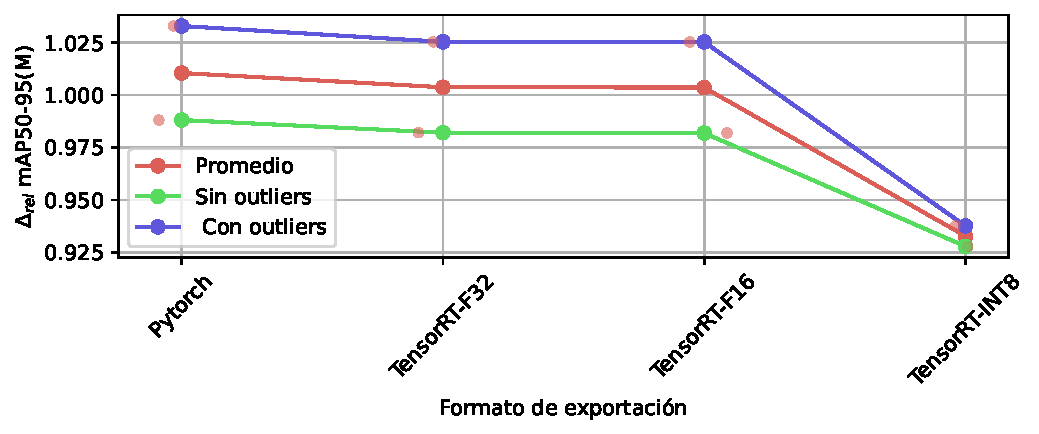
\includegraphics[width=0.9\textwidth]{figures/DeepFish-TransferLearningFactorMejora-Format-mAP50-95(M).pdf}
    \caption{Factor de mejora de usar TransferLearning en Deepfish, por formato de exportación.}
    \label{fig:deepfish_yolo_transfer_learning_factor_mejora}
  \end{subfigure}

  \begin{subfigure}[b]{\textwidth}
    \centering
    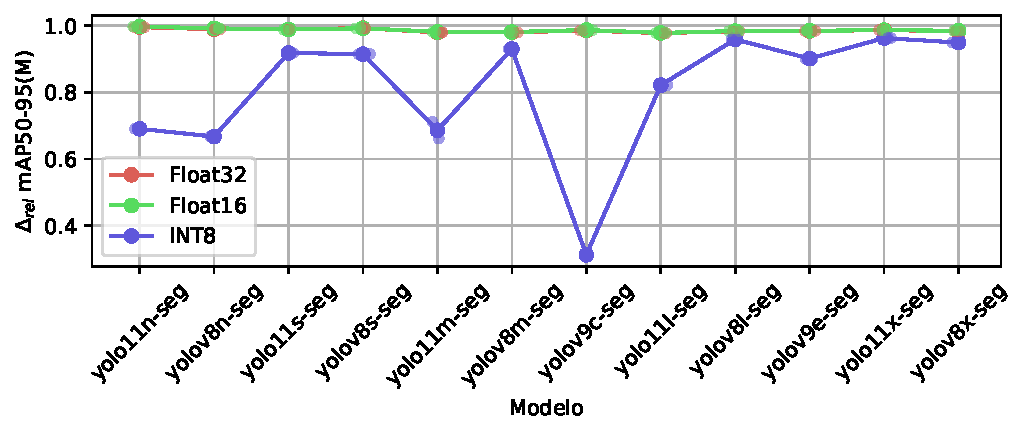
\includegraphics[width=0.9\textwidth]{figures/DeepFish-FormatFactorMejora_TransferLearning-YOLO-mAP50-95(M).pdf}
    \caption{Factor de mejora de exportar a TensorRT por modelo en Deepfish, con Transfer Learning.}
    \label{fig:deepfish_yolo_format_factor_mejora_transfer_learning}
  \end{subfigure}

  \begin{subfigure}[b]{\textwidth}
    \centering
    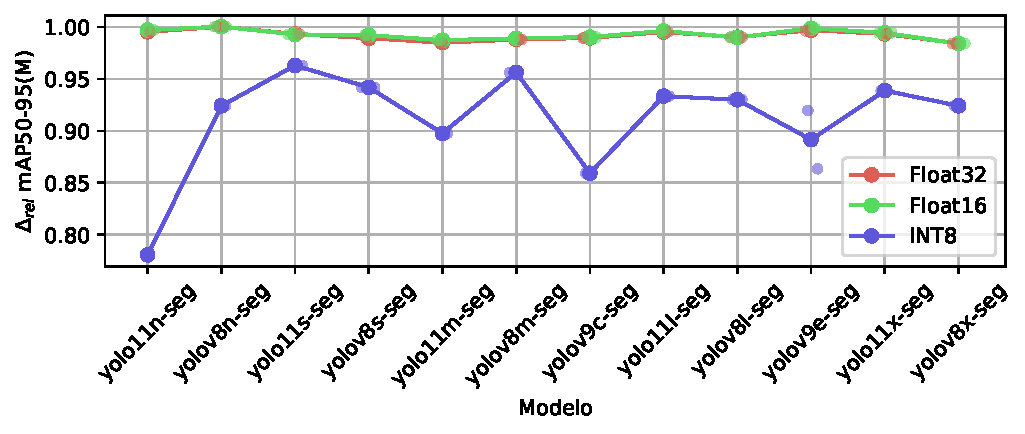
\includegraphics[width=0.9\textwidth]{figures/DeepFish-FormatFactorMejora_FullLearning-YOLO-mAP50-95(M).pdf}
    \caption{Factor de mejora de exportar a TensorRT por modelo en Deepfish, sin Transfer Learning.}
    \label{fig:deepfish_yolo_format_factor_mejora_full_learning}
  \end{subfigure}

  \caption[Factor de mejora de pasar de PyTorch a TensorRT en Deepfish]{Factor de mejora de pasar de PyTorch a TensorRT en Deepfish. Valores menores a 1 indican caída de rendimiento.}
  \label{fig:deepfish_yolo_format_factor_mejora}
\end{center}
\end{figure}

\subsection{Búsqueda de hiperparámetros y entrenamiento final}
Con base en los resultados obtenidos en el entrenamiento inicial, se diseñó una configuración apropiada para realizar búsqueda de hiperparámetros. Como hiperparámetros base se dejaron los valores por defecto de Ultralytics. Para la búsqueda se utilizó el espacio de búsqueda detallada en la tabla \ref{tab:search_space}, y se empleó la librería Raytune \cite{Raytune}.

\begin{itemize}
    \item \textbf{Transfer Learning}: aunque mejoró mAP50 y F1, no se empleó en el entrenamiento final, pues permitir la adaptación completa del modelo (sin congelar capas) es clave para maximizar mAP50-95 y reducir la degradación al exportar a TensorRT.
    \item \textbf{Optimizador}: se escogió SGD, que superó a AdamW, mostró mejor convergencia y menor degradación al exportar a TensorRT.
    \item \textbf{Versión del \textit{dataset}}: se usa la versión completa de Deepfish; la inclusión de imágenes de fondo aportó una mejora marginal y ayudó a mitigar la degradación al exportar a TensorRT.
    \item \textbf{Modelos}: se priorizan modelos grandes por su mejor comportamiento en mAP50-95: YOLOv8l, YOLOv8x, YOLOv9e, YOLO11l y YOLO11x.
\end{itemize}

\begin{table}[htbp]
\centering
\caption[Espacio para la búsqueda de hiperparámetros con Raytune]{Espacio para la búsqueda de hiperparámetros con Raytune.}
\label{tab:search_space}
\begin{tabular}{|c|c|c|}
\hline
\textbf{Hiperparámetro} & \textbf{Rango de búsqueda} & \textbf{Descripción} \\ \hline
lr0 & (1e-4, 0.01) & initial learning rate \\ \hline
lrf & (0.01, 0.5) & factor for final learning rate (lr0 * lrf) \\ \hline
momentum & (0.6, 0.98) & SGD momentum/Adam beta1 \\ \hline
weight\_decay & (0.0, 0.001) & optimizer weight decay 5e-4 \\ \hline
warmup\_epochs & (0.0, 5.0) & warmup epochs (fractions ok) \\ \hline
warmup\_momentum & (0.0, 0.95) & warmup initial momentum \\ \hline
\end{tabular}
\end{table}

Se realizó una busqueda de 50 entrenamientos por modelo, cada uno de 80 épocas y un tamaño de lote de 6 para YOLOv9e y 8 para los demás. Los mejores hiperparámetros resultantes se ven en la tabla \ref{tab:best_hiperparemters_deepfish}. Luego se seleccionaron los mejores resultados según la métrica mAP@50-95, y se procede a un entrenamiento final de 80 épocas con los mejores hiperparámetros encontrados para cada modelo. Los resultados finales de los modelos entrenados se muestran en la tabla \ref{tab:deepfish_resultados_finales}. 

\begin{table}[htbp]
\centering
\caption{Mejores hiperparámetros de entrenamiento encontrados para Deepfish.}
\label{tab:best_hiperparemters_deepfish}
\resizebox{\textwidth}{!}{
\begin{tabular}{|r|r|r|r|r|r|r|r|}
\hline
\multicolumn{1}{|c|}{\textbf{Model}} & \multicolumn{1}{c|}{\textbf{batch}} & \multicolumn{1}{c|}{\textbf{lr0}} & \multicolumn{1}{c|}{\textbf{lrf}} & \multicolumn{1}{c|}{\textbf{momentum}} & \multicolumn{1}{c|}{\textbf{warmup\_epochs}} & \multicolumn{1}{c|}{\textbf{warmup\_momentum}} & \multicolumn{1}{c|}{\textbf{weight\_decay}} \\ \hline
yolov8l-seg & 8 & 0.003009... & 0.021028... & 0.817695... & 1.812856... & 0.490035... & 0.000961... \\ \hline
yolov8x-seg & 8 & 0.006184... & 0.284491... & 0.747041... & 1.295317... & 0.908111... & 0.000970... \\ \hline
yolov9c-seg & 6 & 0.006843... & 0.119841... & 0.722115... & 0.191734... & 0.649675... & 0.000623... \\ \hline
yolo11l-seg & 8 & 0.003518... & 0.208119... & 0.747114... & 0.311229... & 0.519880... & 0.000468... \\ \hline
yolo11x-seg & 8 & 0.002853... & 0.019204... & 0.700485... & 3.989557... & 0.542153... & 0.000441... \\ \hline
\end{tabular}
}
\end{table}

El mejor F1 fue 0.987081 (YOLOv8l), encima de versiones YOLO previas pero debajo de Mask-RCNN y MS-RCNN ---la búsqueda de hiperparámetros encontró F1 superiores, pero esta no fue la métrica priorizada. El mejor mAP50 alcanzó 0.990494 (YOLO11x), superando todos los SOTA; y el mejor mAP50-95 fue 0.866947 (YOLOv9e), sin referencia previa para comparar. Además, la degradación al exportar a TensorRT-INT8 es consistente con los análisis previos.

\begin{table}[htbp]
\centering
\caption[Métricas de validación finales para Deepfish]{Métricas de validación finales para los modelos entrenados con Deepfish. Los datos en gris corresponden a los mejores resultados en el SOTA encontrados en trabajos anteriores \cite{Guerrero2024}.}
\label{tab:deepfish_resultados_finales}
\resizebox{\textwidth}{!}{
\begin{tabular}{|r|r|r|r|r|r|r|}
\hline
\multicolumn{1}{|c|}{\textbf{Model}} & \multicolumn{1}{c|}{\textbf{precision}} & \multicolumn{1}{c|}{\textbf{recall}} & \multicolumn{1}{c|}{\textbf{F1\_score}} & \multicolumn{1}{c|}{\textbf{mAP50}} & \multicolumn{1}{c|}{\textbf{mAP50-95}} & \multicolumn{1}{c|}{\textbf{Format}} \\ \hline
 & 0.999798 & 0.974684 & 0.987081 & 0.988554 & 0.854858 & Pytorch \\ \cline{2-7} 
\multirow{-2}{*}{yolov8l-seg} & 0.997991 & 0.962025 & 0.979678 & 0.986868 & 0.828008 & TensorRT-INT8 \\ \hline
 & 1.000000 & 0.971526 & 0.985558 & 0.982418 & 0.856800 & Pytorch \\ \cline{2-7} 
\multirow{-2}{*}{yolov8x-seg} & 1.000000 & 0.909706 & 0.952718 & 0.974205 & 0.836648 & TensorRT-INT8 \\ \hline
 & 0.998282 & 0.949367 & 0.973210 & 0.981325 & 0.866947 & Pytorch \\ \cline{2-7} 
\multirow{-2}{*}{yolov9e-seg} & 0.986039 & 0.894078 & 0.937810 & 0.963326 & 0.818743 & TensorRT-INT8 \\ \hline
 & 0.996304 & 0.962025 & 0.978865 & 0.984134 & 0.851774 & Pytorch \\ \cline{2-7} 
\multirow{-2}{*}{yolo11l-seg} & 0.972137 & 0.883325 & 0.925606 & 0.928226 & 0.743149 & TensorRT-INT8 \\ \hline
 & 0.999076 & 0.974684 & 0.986729 & 0.990494 & 0.858102 & Pytorch \\ \cline{2-7} 
\multirow{-2}{*}{yolo11x-seg} & 0.997386 & 0.974684 & 0.985904 & 0.981660 & 0.815214 & TensorRT-INT8 \\ \hline
\rowcolor[HTML]{d4d4d4} 
Mask-RCNN & - & - & 0.989500 & 0.988000 & - & Pytorch \\ \hline
\rowcolor[HTML]{d4d4d4} 
MS-RCNN & - & - & 0.988500 & 0.986000 & - & Pytorch \\ \hline
\rowcolor[HTML]{d4d4d4} 
SOLOv2 & - & - & 0.982900 & 0.975000 & - & Pytorch \\ \hline
\rowcolor[HTML]{d4d4d4} 
Yolov8l-seg* & - & - & 0.944900 & 0.942000 & - & Pytorch \\ \hline
\rowcolor[HTML]{d4d4d4} 
Yolov8x-seg* & - & - & 0.923700 & 0.961000 & - & Pytorch \\ \hline
\end{tabular}
}
\end{table}

\subsubsection{Consideraciones y conclusiones}
Se logra superar el SOTA establecido en el trabajo de \cite[Alejandro Guerrero, 2024]{Guerrero2024}, y se demuestra la viabilidad del uso de exportación a TensorRT para optimizar tiempos de inferencia en aplicaciones en tiempo real, con minima perdida de desempeño.

Cabe mencionar que la versión del \textit{dataset} Deepfish utilizada en este trabajo difiere ligeramente de la empleada en \cite{Guerrero2024}, ya que este incluía instancias de peces combinados (dos peces compartiendo una sola máscara), mientras que en este trabajo se arregló este problema y se separaron en instancias individuales. Esto puede, en parte, explicar diferencias en los resultados obtenidos.